\documentclass{../source/zjureport}

\major{信息工程}
\name{周灿松、王瑜昕、朱夏瑜}
\title{波导实验}
\college{信息与电子工程学院}
\date{\today}
\lab{东4-227}
\stuid{3190105055}
\course{电子电路设计实验}
\instructor{王子立、金向东、龚淑君}
\grades{}
\expname{数控恒流源设计}
\exptype{设计实验}
\partner{}

\begin{document}
    \makecover
    \makeheader

    \section{系统方案}
        \subsection{系统总体框图}

        \begin{figure}[thp]
            \centering
            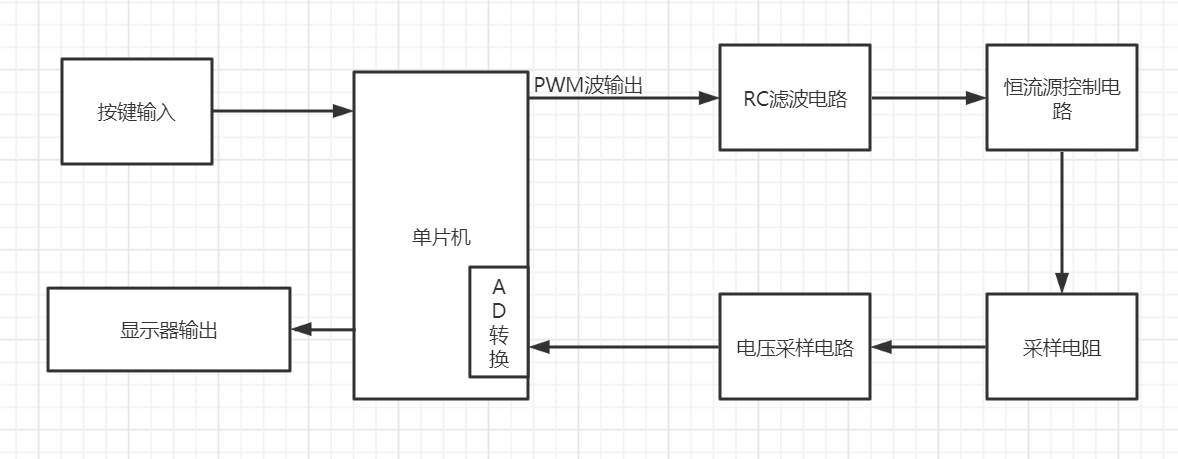
\includegraphics[width = 0.9\textwidth]{figure/系统框图.png}
            \caption{系统总体框图}
        \end{figure}

        \subsection{方案比较与选择}
            \subsubsection{采用开关电源的恒流源}

            采用开关电源的恒流源电路如图1所示。当电源电压降低或负载电阻R1降低时,采样电阻RS上的电压也将减少,则SG3524的12、13管脚输出方 波的占空比增大,从而BG1导通时间变长,使电压U0回升到原来的稳定值。BG1关断后,储能元件L1、E2、E3、E4保证负载上的电压不变。当输入电源电压增大或负载电阻值增大引起U0增大时,原理与前类似,电路通过反馈系统使U0下降到原来的稳定值,从而达到稳定负载电流I1的目的。

            优点:开关电源的功率器件工作在开关状态,功率损耗小,效率高。与之相配套的散热器体积大大减小,同时脉冲变压器体积比工频变压器小了很多。因此采用开关电源的恒流源具有效率高、体积小、重量轻等优点。

            缺点:开关电源的控制电路结构复杂,输出纹波较大,在有限的时间内实现比较困难。
            \newpage

            \begin{figure}[thp]
                \centering
                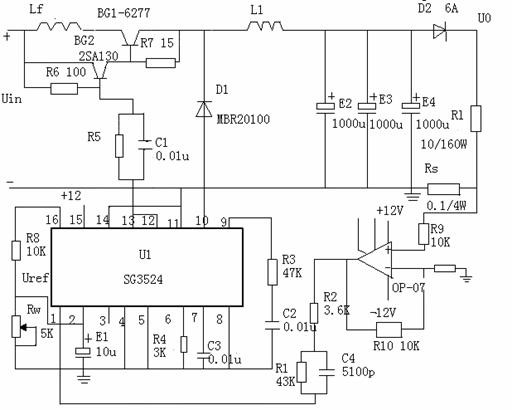
\includegraphics[width = 0.8\textwidth]{figure/采用开关电路的恒流源.jpg}
                \caption{采用开关电源的恒流源}
            \end{figure}

            \subsubsection{采用集成稳压器构成的开关恒流源}
            系统电路构成如图2所示。MC7805为三端固定式集成稳压器,调节RW,可以改变电流的大小,其输出电流为:IL=(UOUT/RW)+I4,式中I4为MC7805的静态电流,小于10mA。当RW较小即输出电流较大时,可以忽略 ,当负载电阻RL变化时,MC7805改变自身压差来维持通过负载的电流不变。

            优点:该方案结构简单,可靠性高
  
            缺点:无法实现数控。

            \begin{figure}[thp]
                \centering
                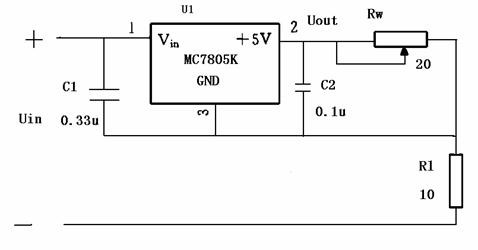
\includegraphics[width = 0.5\textwidth]{figure/采用集成稳压器的开关恒流源.jpg}
                \caption{采用集成稳压器构成的开关恒流源}
            \end{figure}

            \subsection{采用单片机控制的恒流源}
            该方案恒流源电路由N沟道的MOSFET、高精度运算放大器、采样电阻等组成,其电路原理图如图3所示。利用功率MOSFET的恒流特性,再加上电流反馈电路,使得该电路的精度很高。

    
            该电流源电路可以结合单片机构成数控电流源。通过键盘预置电流值,单片机输出相应的数字信号给D/A转换器,D/A转换器输出的模拟信号送到运 算放大器,控制主电路电流大小。实际输出的电流再通过采样电阻采样变成电压信号,A/D转换后将信号反馈到单片机中。单片机将反馈信号与预置值比较,根据 两者间的差值调整输出信号大小。这样就形成了反馈调节,提高输出电流的精度。本方案可实现题目要求,当负载在一定范围内变化时具有良好的稳定性,而且精度较高。
            \begin{figure}[thp]
                \centering
                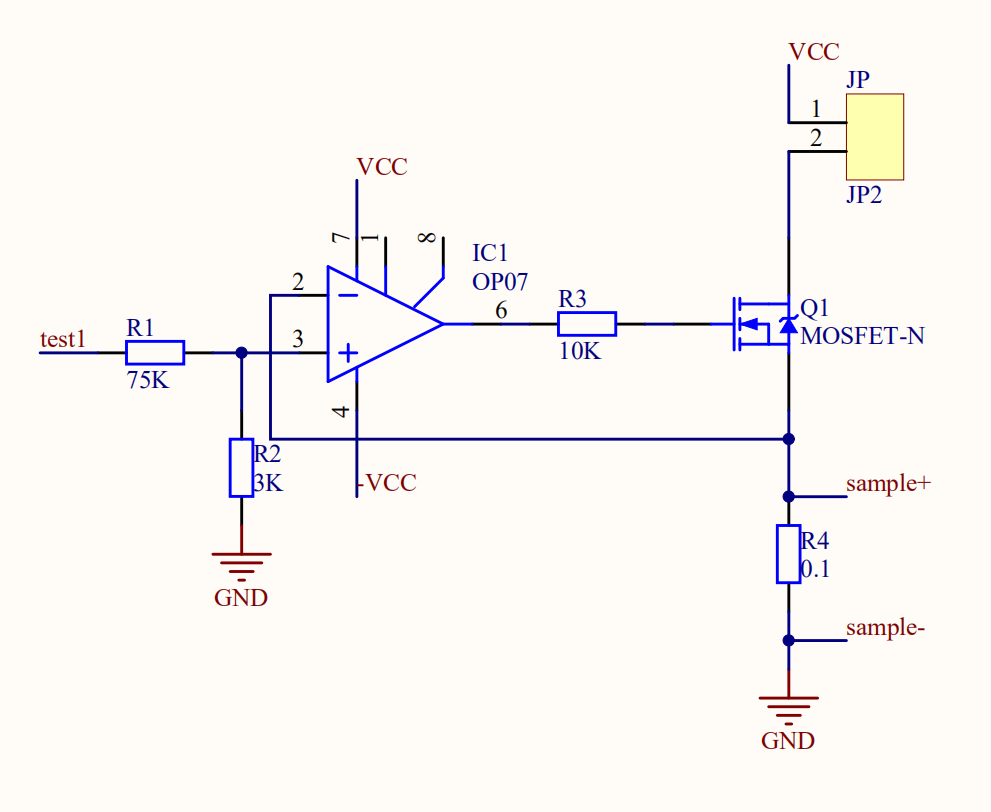
\includegraphics[width = 0.5\textwidth]{figure/采用单片机控制的恒流源.png}
                \caption{采用单片机控制的恒流源}
            \end{figure}

        \subsection{方案描述}

        该数控恒流源电路主要包括按键输入、LCD显示屏输出、单片机、RC滤波电路、压控恒流源电路、电压采样电路几个模块。

        系统工作原理为:通过按键对电流值S_CURRENT进行预置,并显示在LCD显示屏上,单片机根据预置的电流值输出一定占空比的PWM波,通过RC滤波电路后输出直流信号。直流信号输送至压控恒流源模块,通过电阻分压后输送至大功率场效应管IRF640,产生相应的电流值。场效应管的漏极电流即为恒流源的实际输出电流。场效应管的漏极电流近似于源极电流,在电压采样模块,场效应管的源极电流经过采样电阻后转化为电压信号,经过差分放大电路后输送至单片机,单片机采集此信号,作出相应的调整处理后输出显示在LCD显示屏上,作为电流源的自测表的输出值N_CURRENT,实际的输出电流通过电流表测量得到。

    \section{理论分析与计算}
        \subsection{理论分析}
        我们组的电路主要分为3个部分,恒流控制电路,采样放大电路,单片机电路,这里主要对恒流控制电路和采样放大电路进行介绍分析。

        恒流控制电路主要用于控制一个恒定的电流进行输出,首先根据你设定的值控制单片机输出一个占空比确定的pwm波,pwm波经过RC滤波变为一个恒定的电压,也就是经过pwm输出电路,此时这个确定的电压值在经过分压进入恒流控制电路,这里进行分压的原因主要由于我们所取的采样电阻比较小,因此必须控制输入的电压值,经过确定分压比之后的电压再进入运算放大器,根据理想运放的特性我们可以指导,2、3两脚的电压值近似相等,而2脚又与采样电阻相连,因此此时完整的电压进入采样电阻,采样电阻另一端又接地,因此此时采样电阻上的电流即为分压后的电压除以采样电阻的阻值,而根据mos管的特性,运算放大器和mosfet相连出来的电流可以近似忽略,因此采样电阻上的电流值与我们的输出接口JP JP2上的电流值相等,而据此可知,我们可以控制pwm波的占空比来线性地控制电流。

        而电压采样电路主要起到一个放大反馈的作用,采样电阻上的电压进入我们的电压采样电路,而根据电压采样电路上的电阻阻值,我们可以确定一个恒定的放大比,在这个电路中,我们把R7、R8的值设定为相等,R9、R10的值也设定为相等,最后得到的放大比例即为两者之比,放大后的电压后输出到AD输入电路,此时对放大后的电压进行RC滤波,之后将这个滤波后的电压输入到单片机的Adin,单片机根据输入进来的Adin可以进行数模转化,而数模转化比较后则可以对单片机的pwm占空比进行一个调节,以此来达到一个反馈调节的功能。

        至于电源模块,LCD电路我们则是根据老师所给的单片机学习板而设计,两者相吻合以此来保证正确性,我们也适当删减了一些单片机学习板上一些没有必要的电路。

        恒流控制电路和电压采样电路我们主要参考了老师放在群里的资料。

        \subsubsection{理论计算}
        电路中主要需要计算的是恒流控制电路和电压采样电路的一些电阻值。
   
        这里我先对恒流控制电路上的分压比进行计算,一开始在不知道采样电阻只能是0.1欧姆之前,我们是按照0.15欧姆来进行计算的,不过此处我就根据0.15欧姆的思路给出0.1欧姆的计算思路,首先是分压比调控,因为pwm波的占空比只能在256个值之内进行调节,因此我们取了一个比较好的占空比也即为200,因此我们设定它的满量程也即是实验要求20mA到1000mA,满量程对应此,1000mA在采样电阻对应0.15V,而pwm最大的电压量为5V,因此5V*k*200/256=0.15,据此我们可以得到k=0.0384,而根据标称电阻值,我们得到了两个电阻值是比较符合的,3K欧姆和75K欧姆,3/75+3我们可以得到也为0.384,因此这就是我们在横流控制电路上的计算。
  
        然后我们对于电压采样电路上的电阻值进行计算,此处我们采用了相同的电阻值进行控制,也就是R7=R8=3K,而R9=R10=75K,而根据运放的特性我们可以得到放大的比例为R9/R7=25,因此我们对于采样电阻上的电压放大了25倍。之后的一些电容值我们根据老师所给的资料以及老师之后的建议我们进行了调节,最后所得到的电容值如之前的电路图所示。
  
        此时我们已经可以完整的量程范围(20, 1000)mA,而采样电阻上的电压值的范围为(3,150)mV,再到分压前的电压为(78,3900)mV,最后根据此得到占空比(,0.0156,0.78),对应有占空比的分子(4,200)。
  
        而在最后电路板的焊接过程中,我们又进行了调节,采样电阻改为了0.1欧姆,而在实验室的柜子中75K欧姆的电阻是不存在的,因此我们采取了100K欧姆的电阻进行了代替,当然根据我们电路板的测试中,在Adin电路和pwm输入电路中,本身就存在一定的压降,因此我们最后还是根据实际测出来pwm值,AD值,以及实际电流值,来对我们程序内部的参数来进行设计。
        \newpage

    \section{电路与程序设计}
        \subsection{硬件电路设计}
            \subsubsection{各模块电路}
            \begin{enumerate}
                \item 总体电路
                \begin{figure}[thp]
                    \centering
                    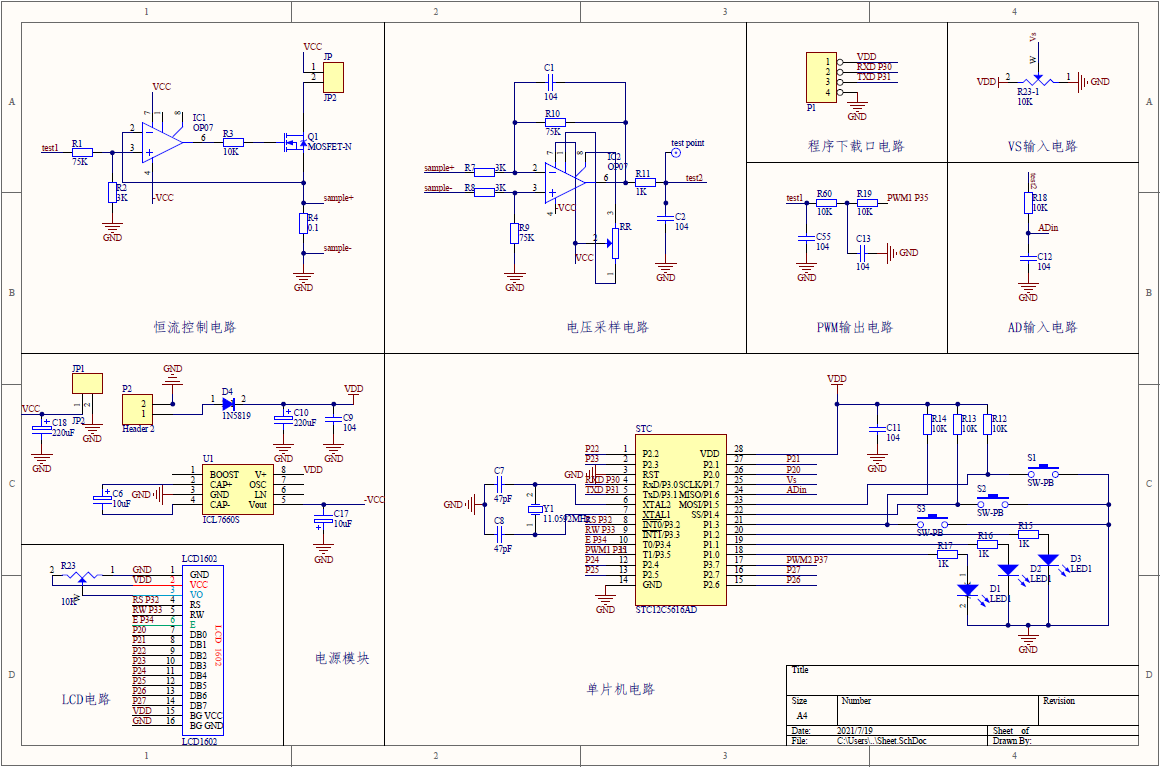
\includegraphics[width = 0.8\textwidth]{figure/总体电路.png}
                    \caption{总体电路}
                \end{figure}
                \item 压控恒流源模块
                
                压控恒流源是该系统的主要部分,通过电压来控制输出电流的变化。该压控恒流源电路由分压电阻R1、R2,运算放大器IC1,大功率场效应管Q1,采样电阻R4,电流输出模块JP2等组成。

                压控恒流源电路的工作原理为:输入RC滤波电路得到的直流信号,经过分压后得到U3输入运算放大器,控制输出对应的电流Io。运放采用OP-07作为电压跟随器,由于U2=U3,场效应管Id=Is,可以得到Io=Is=U2/R53= U3/R53。从Io=U3/R53可以看出,电路输入电压U3控制输出电流Io,即Io不随RL的变化而变化,从而实现压控恒流。
                \newpage
                \begin{figure}[thp]
                    \centering
                    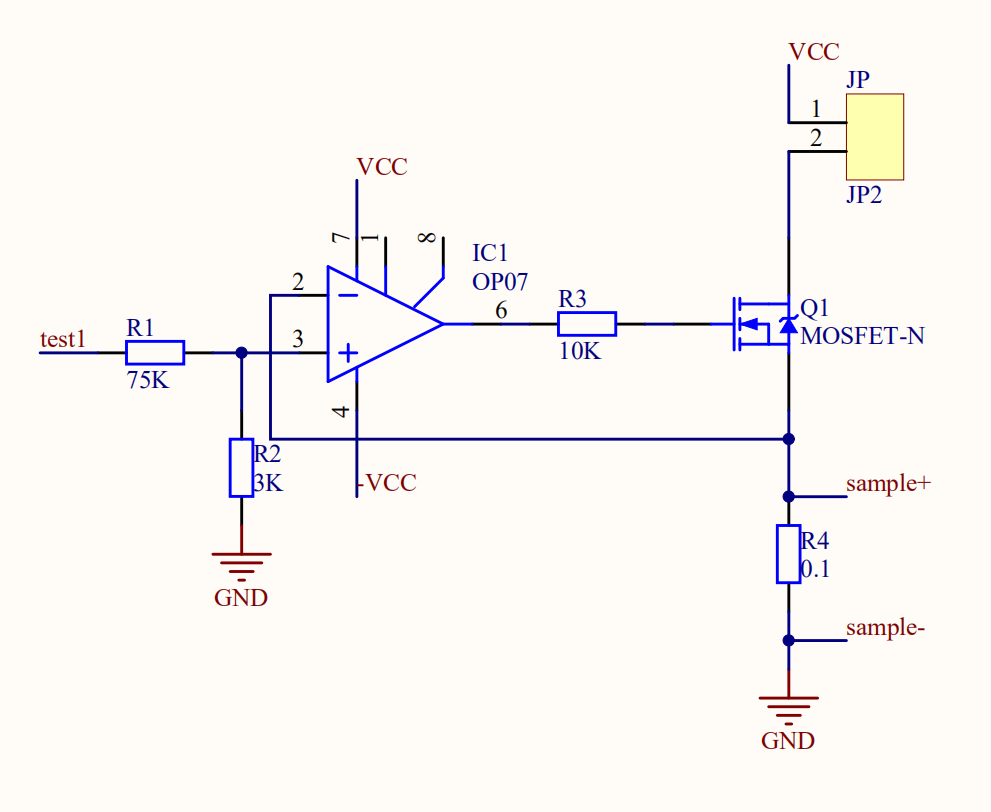
\includegraphics[width = 0.5\textwidth]{figure/压控恒流源模块.png}
                    \caption{压控恒流源模块}
                \end{figure}
                \item 电压采样模块
                
                电压采样模块是反馈部分。该电压采样模块采用差分放大电路,由运算放大器IC2、若干电阻电容组成。电路原理图如图7所示。

                其工作原理为:对采样电阻R4上的电压进行采样,经放大后输入单片机,由单片机内部的ADC模块转换为数字信号作为反馈,PID调整输出的PWM波,实现负反馈。
                \begin{figure}[thp]
                    \centering
                    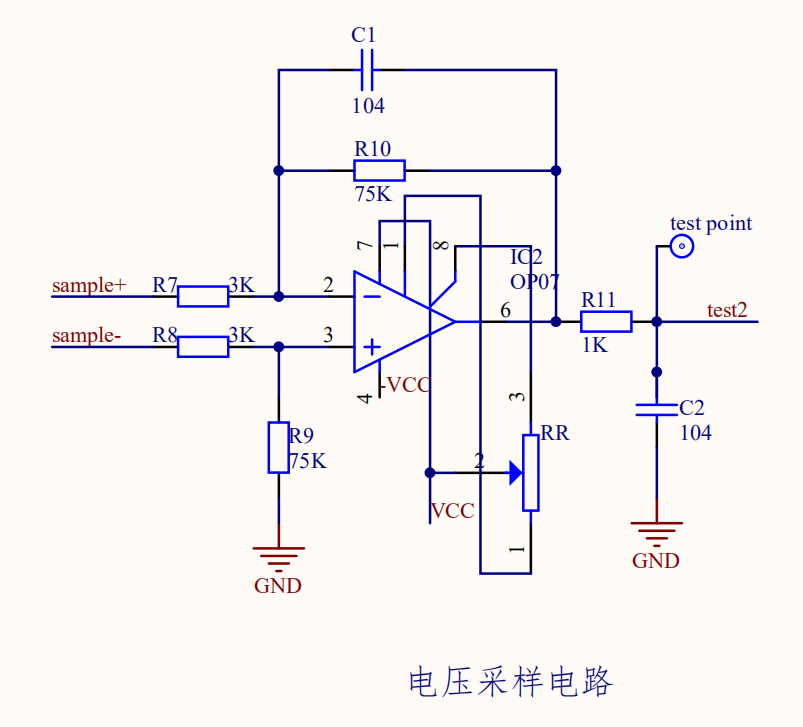
\includegraphics[width = 0.5\textwidth]{figure/电压采样模块.png}
                    \caption{电压采样模块}
                \end{figure}
                \item 按键输入模块
                
                该模块采用三个按键输入,按键1控制改变数字的位,按键2控制数字+1,按键3为确认输入,将设定的数字输入单片机。按键采用防抖动设计。
                \item 单片机以及A/D转换模块
                
                单片机为本系统的主控制器,本次设计采用型号为STC1C5410AD的单片机,指令周期短,工作速率快,功耗低,具有丰富的片上资源,可以在线下载,易于调试。

                单片机自带的A/D转换模块为10位,取高八位为有效位,转换模块将输入的采样电压转换成数字信号反馈给单片机,单片机将此反馈信号与预置值比较,根据两者间的差值调整输出信号大小。这样就形成了反馈调节,提高输出电流的精度。同时,将采样回来的电压经过单片机处理传送到LCD,可以显示当前的实际电流值。

                \begin{figure}[thp]
                    \centering
                    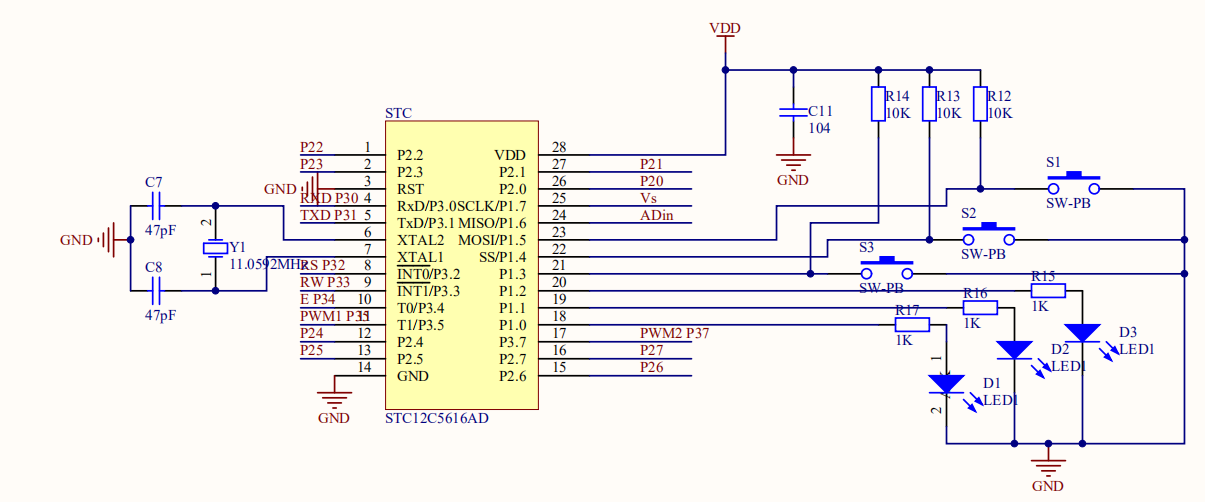
\includegraphics[width = 0.7\textwidth]{figure/单片机电路.png}
                    \caption{单片机电路}
                \end{figure}
                \item LCD显示模块
                
                LCD显示屏型号为LCD1602,第一行显示设定电流值S_CURRENT,第二行显示单片机测量值N_CURRENT。

                \begin{figure}[thp]
                    \centering
                    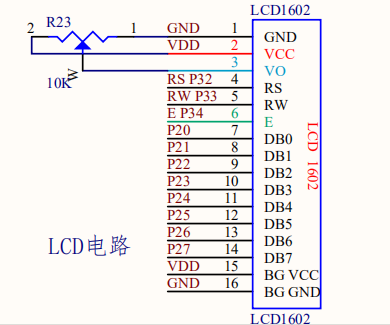
\includegraphics[width = 0.5\textwidth]{figure/LCD电路.png}
                    \caption{LCD电路}
                \end{figure}
                \item 电源模块
                
                电源模块由学生电源提供12V直流,由ICL7660S生成-5V的电压。
                \newpage
                \begin{figure}[thp]
                    \centering
                    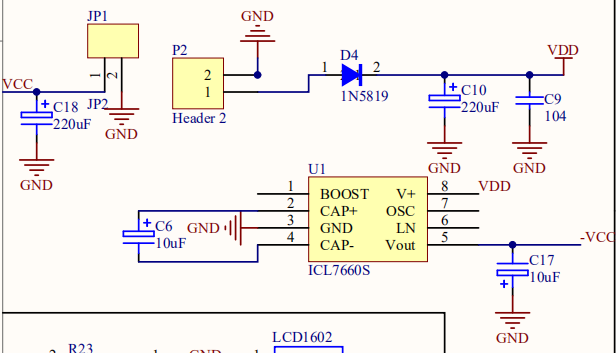
\includegraphics[width = 0.5\textwidth]{figure/电源模块.png}
                    \caption{电源模块}
                \end{figure}
            \end{enumerate}
            \subsubsection{PCB设计}
            \begin{figure}[thp]
                \centering
                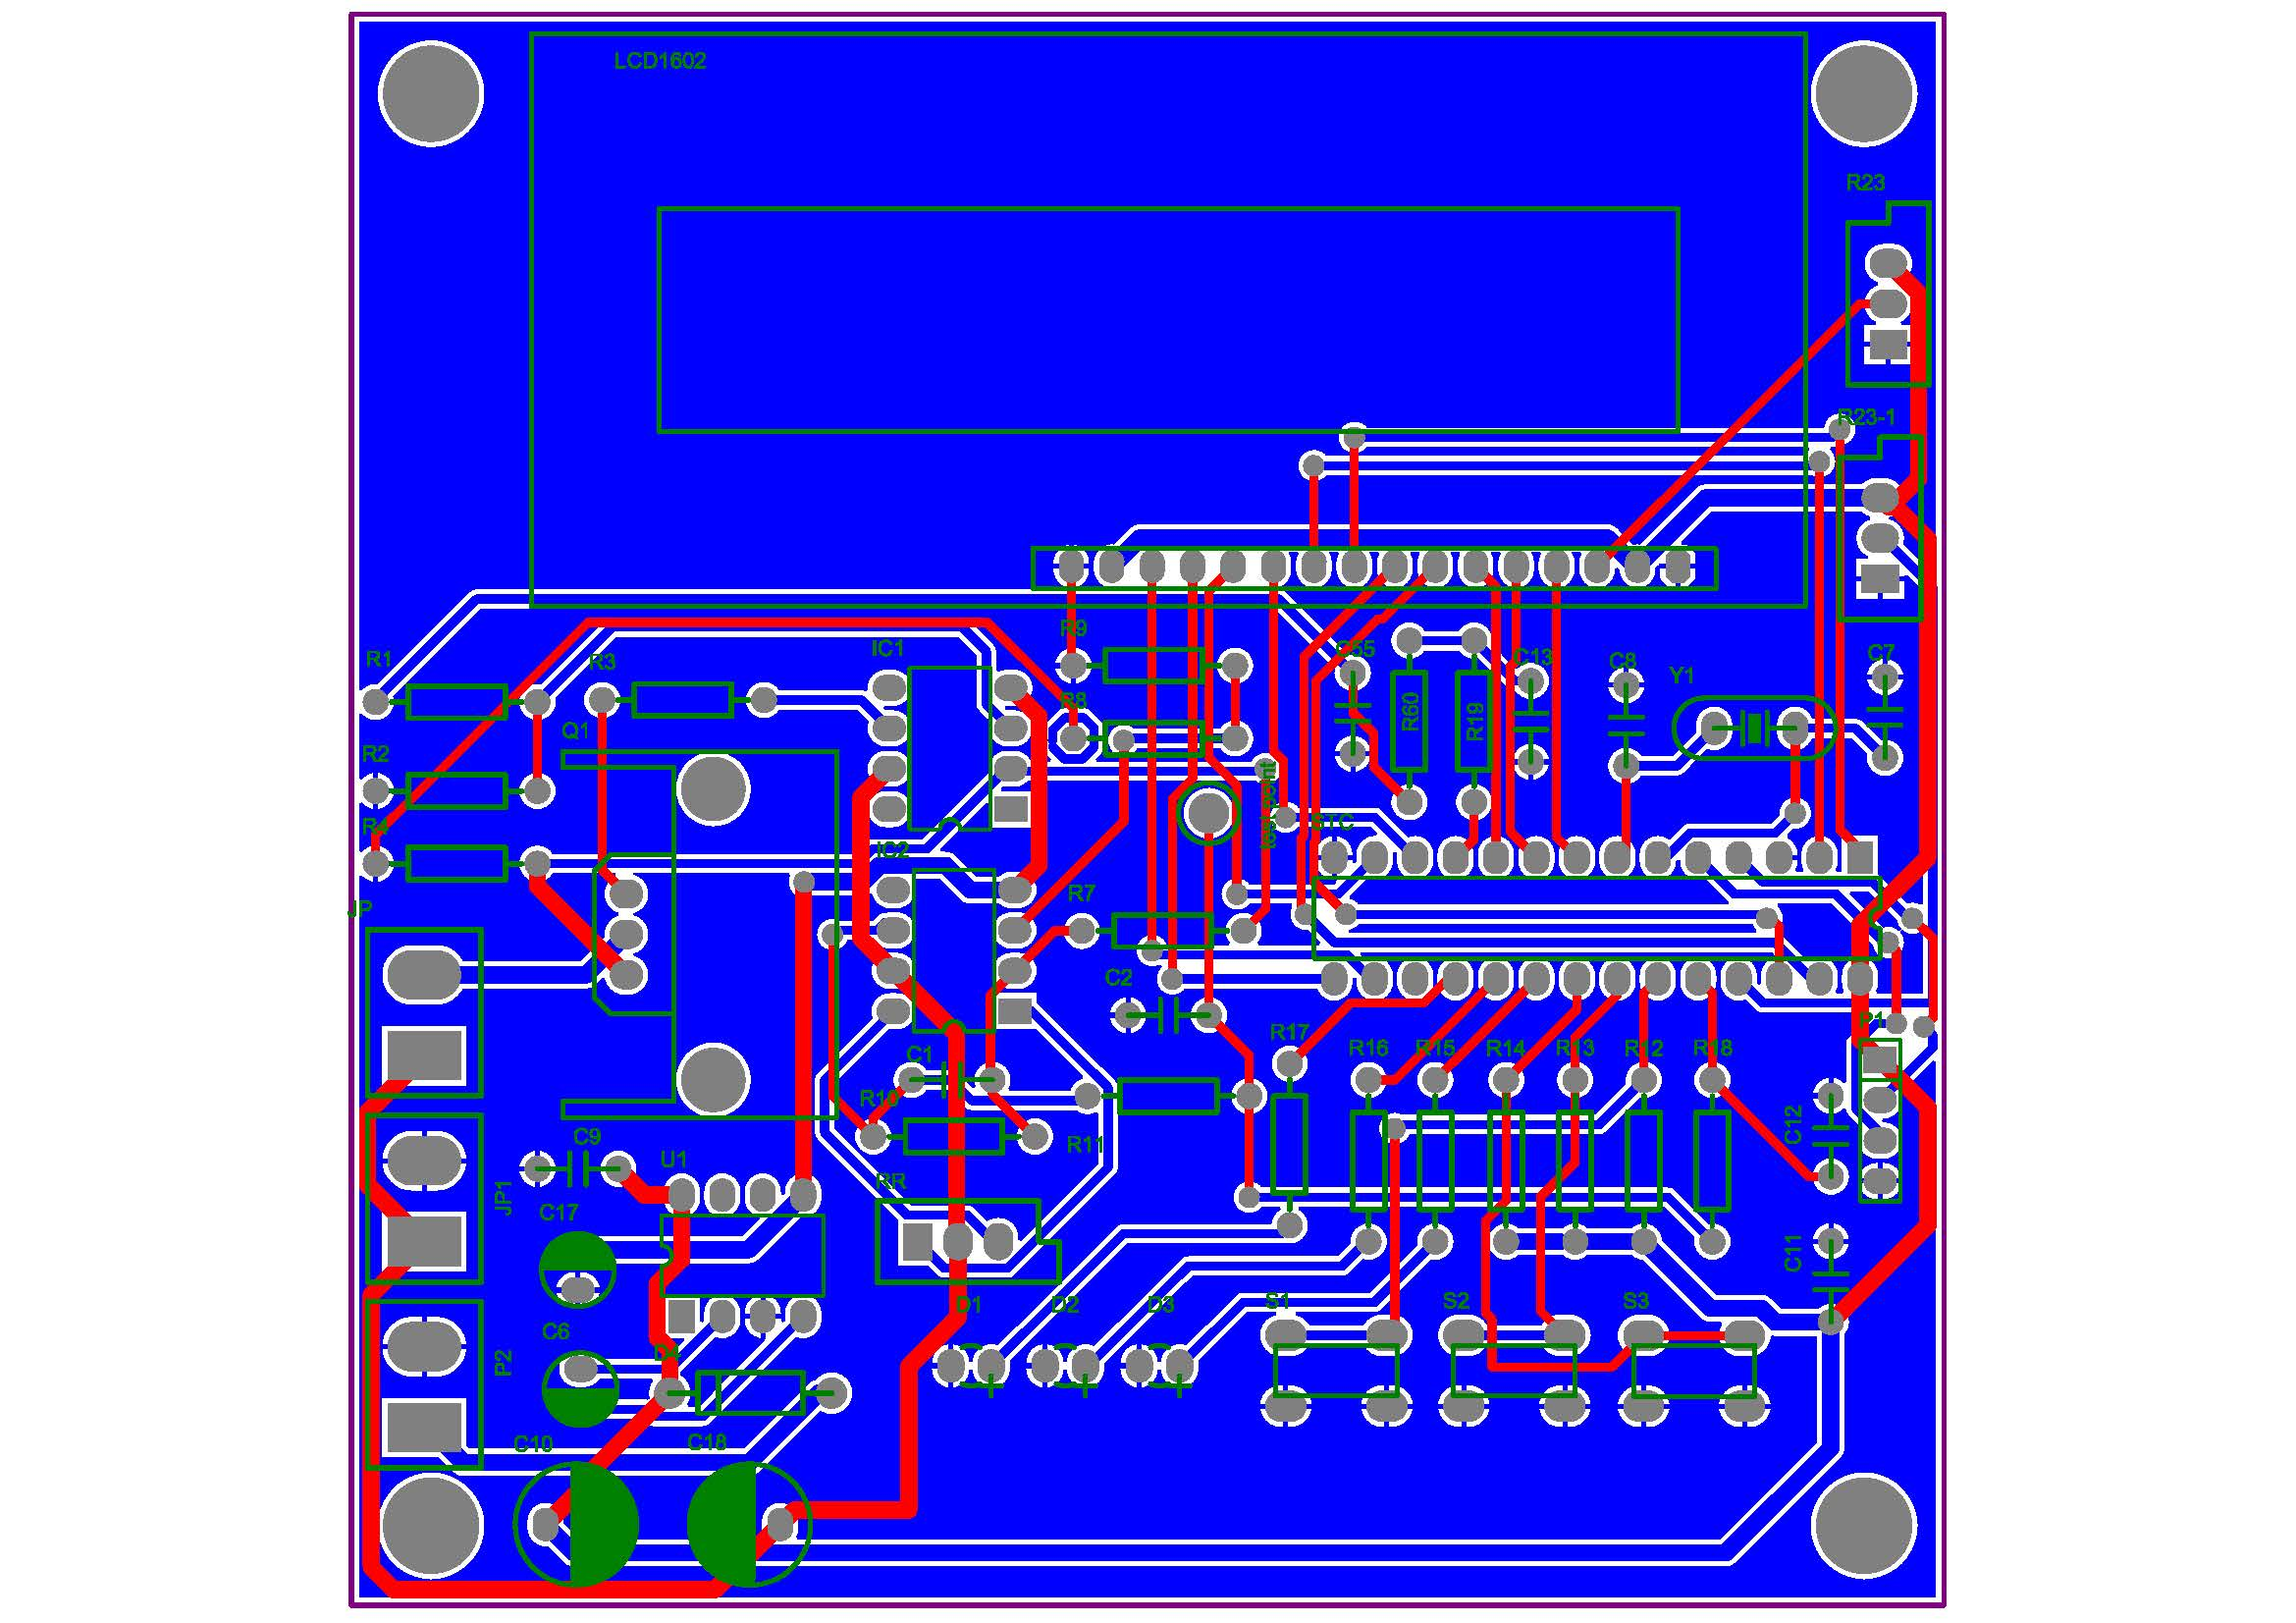
\includegraphics[width = 0.8\textwidth]{figure/PCB.jpg}
                \caption{PCB设计}
            \end{figure}
            \newpage
        \subsection{软件设计}
            \subsubsection{流程图}

            \begin{figure}[thp]
                \centering
                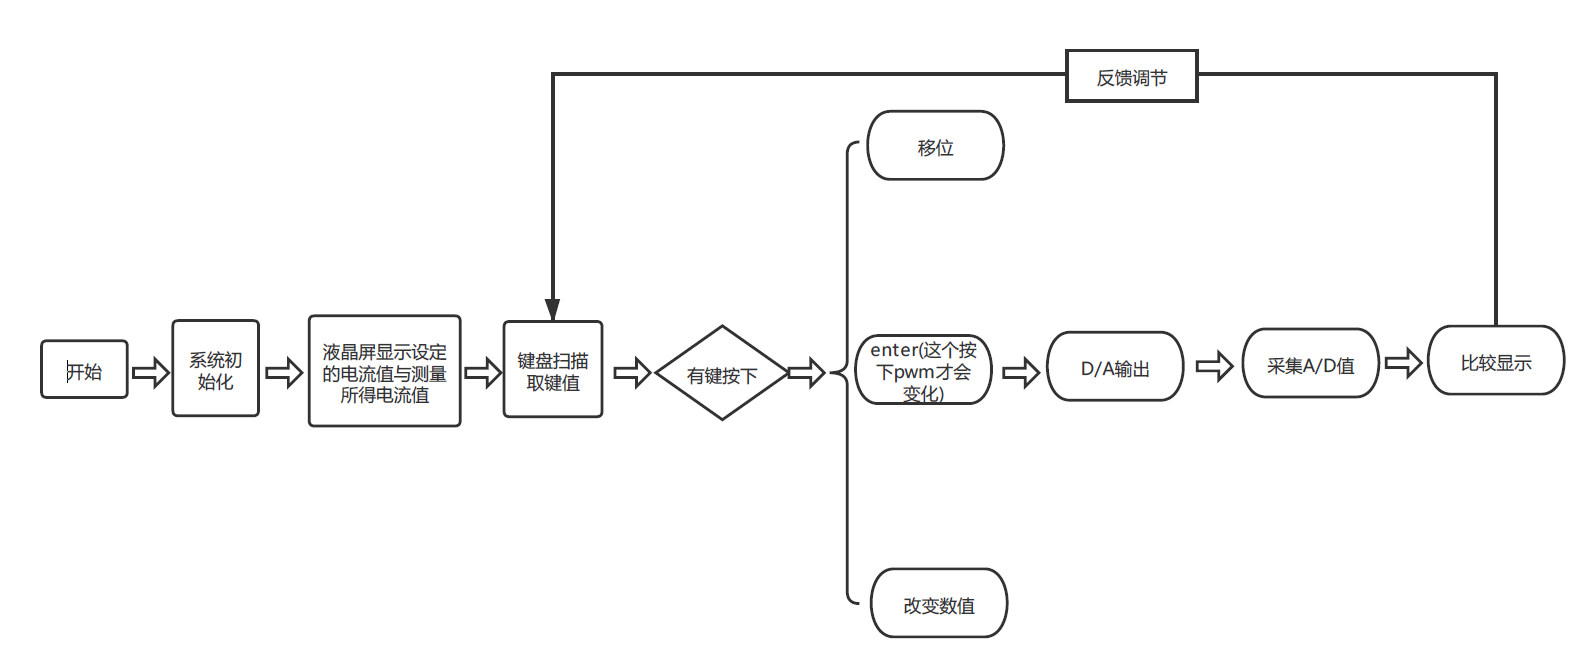
\includegraphics[width = 0.8\textwidth]{figure/软件框图.png}
                \caption{流程图}
            \end{figure}
            \subsubsection{模块核心代码}
            \begin{lstlisting}[
                caption=ADC输入及转换为实际电流,
                language = C
                ]
            void ADC_Scan(){
            //开启ADC,通道六扫描
            ADC_CONTR = ADC_POWER | ADC_SPEEDLL | 6 | ADC_START;
            _nop_();                        //Must wait before inquiry
            _nop_();
            _nop_();
            _nop_();
            while (!(ADC_CONTR & ADC_FLAG));//Wait complete flag
            ADC_CONTR &= ~ADC_FLAG;         //Close ADC
            //将10位转换结果存入Adc_resuit变量
            Now_Current = ADC_DATA*4+(ADC_LOW2 && 0x03);
                
            //将电流转换为实际电流值
            Now_Current = Now_Current/0.65;
                    
                }
            \end{lstlisting}
            \newpage
            \begin{lstlisting}[
                caption = 按键操作及PWM控制,
                language = C
            ]
            void	Key_treat()
            {
                if (Key3_press_flag)
                {
                    //将预设值传入PWM
                    result = Set[3]*1000 + Set[2]*100 + Set[1]*10 + Set[0];
                    //将按键输入结果转化为PWM控制值
                    result = 255 - result/gain;
                    Key3_press_flag = 0;
                }
            
                if (Key2_press_flag)
                {
                    switch (target)
                    {	
                    case 0: Set[3-target] = (Set[3-target] + 1)%2;
                        break;
                    
                    default: Set[3-target] = (Set[3-target] + 1)%10;
                        break;
                    }
                    Key2_press_flag = 0;
                }
            
                if (Key1_press_flag)
                {
                    target = (target+1)%4;
                    Key1_press_flag = 0;
                }
            
            }
            \end{lstlisting}
            \newpage
    \section{测试方案与测试结果}
        \subsection{测试步骤}
        \begin{enumerate}
            \item 单片机PWM波输出占空比设置为50\%,改变负载,测试恒流控制模块是否能达到恒流控制效果
            \item  断开PWM波反馈回路,测量单片机ADC输入,得到输出电流与ADC转换结果之间的关系,校准参数
            \item 连接PWM反馈回路,设定不同的电流值,计算得到PWM占空比与电流之间的关系,调整代码
        \end{enumerate}
        
        \subsection{测试结果}
            \subsubsection{电流范围与步进调节}
            \begin{table}[thp]
                \centering
                \begin{tabular}{|c|c|c|c|c|c|c|}
                \hline
                设定值(mA) & 20   & 30   & 40   & 50   & 500   & 1000   \\ \hline
                测定值(mA) & 19.7 & 29.4 & 39.1 & 48.4 & 498.5 & 1003.1 \\ \hline
                显示值(mA) & 20   & 26   & 38   & 44   & 493   & 998    \\ \hline
                \end{tabular}
                \end{table}
            \subsubsection{负载电阻改变电流变化测量}
            \begin{table}[thp]
                \centering
                \begin{tabular}{|c|c|c|}
                \hline
                \multicolumn{3}{|c|}{设定500mA} \\ \hline
                接入电阻    & 第一次测量    & 第二次测量    \\ \hline
                0欧姆     & 498.5mA  & 500.1mA  \\ \hline
                7.5欧姆   & 493.1mA  & 495.5mA  \\ \hline
                \end{tabular}
                \end{table}

            \subsubsection{纹波电流测量}
            接入7.5Ω电阻,将示波器接在电阻两端,得到文波电流为2mA
        \subsection{数据处理}
        \begin{table}[htp]
            \centering
            \begin{tabular}{|c|c|c|c|c|c|c|}
            \hline
            设定值(mA) & 20   & 30   & 40   & 50   & 500   & 1000   \\ \hline
            测定值(mA) & 19.7 & 29.4 & 39.1 & 48.4 & 498.5 & 1003.1 \\ \hline
            显示值(mA) & 20   & 26   & 38   & 44   & 493   & 998    \\ \hline
            设定与测量差值 & 0.3  & 0.6  & 0.9  & 1.6  & 1.5   & -3.1   \\ \hline
            测量与显示差值 & -0.3 & 3.4  & 1.1  & 4.4  & 5.5   & 5.1    \\ \hline
            \end{tabular}
            \end{table}

            \begin{table}[htp]
                \centering
                \begin{tabular}{|c|c|c|}
                \hline
                \multicolumn{3}{|c|}{设定500mA} \\ \hline
                接入电阻     & 第一次测量    & 第二次测量   \\ \hline
                0欧姆      & 498.5    & 500.1   \\ \hline
                7.5欧姆    & 493.1    & 495.5   \\ \hline
                变化值      & 5.4      & 4.6     \\ \hline
                \end{tabular}
                \end{table}
                \newpage
        \subsection{数据分析}
            \subsubsection{电流范围与步进}
            由上述表格可知,我们能够通过设定不同的值使输出电流在20mA~1000mA的范围内变化,步进至少能达到10mA的精度,达到了基础部分对步进的要求,同时电流可调范围达到了提升要求部分。
            \subsubsection{输出电流与给定值偏差}
            由上述表格可知,设定不同的输出电流时,测量电流与设定值之间的最大差值出现在设定1000mA时,为3.1mA,远远小于要求中的设定值的1\%+10mA
            \subsubsection{显示输出与电流差值}
            由上述表格可知,显示值与测量差值之间的误差最大发生在设定电流为500mA时,差值为5.5mA,要求允许的最大差值为$(1000\times 1\%+3)mA = 13mA$,满足要求
            \subsubsection{改变负载电阻}
            我们将电流输出设定为500mA,由表三可知,空载时输出电流与接入负载后输出电流变化值在2mA左右,而要求中的变化值为3mA,符合系统设计要求
            \subsubsection{文波系统}
            测量出的文波电流为2mA,达到了基础要求中的5mA,但是没有达到提升部分中的1mA要求

            \newpage
        
    \section{实验的心得体会}
        \subsection{王瑜昕}
        这次的小学期实验令我收获很大,学期内的电子电路设计实验因为当时选了一个比较容易的题目,,用arduino做一个不同量程的电容测量仪,如果不算arduino和lcd1602,整个电路图只有一些电阻电容,非常的简单,因此也可以料想到之后的设计电路图和pcb版图绘制比较简单,同时当时的实验老师对于pcb版图的绘制线的绘制覆铜等的要求都是比较低的,因此,这次的小学期实验反而是更令我完整的走了一遍从设计到制作的流程。

        在这次的小学期中遇到了许许多多的问题,但也慢慢的将他们都解决了,首先我们的电路设计总体来说还是比较顺利的,因为老师已经给出了参考电路图,我们根据老师给出的参考电路图将其进行整合优化设计,但由于我们审题的不仔细,未注意题目要求是只有一个12V电压的供电,因此我们在设计时,默认了我们可以使用负电源,导致终稿提交时出现失误,同时在准备负电源的时候我们也找到了对应的芯片专门用于产生负电压,也知道了它也是有范围限制,同时在电路设计的时候也明白了滤波电容的重要性,一般来说,例如你的pwm波或者说之后进去的ad_in等,都是需要添加滤波电容来保证电源的稳定性,在设计过程中,对于电路分模块的理解进一步加深了。

        这次的PCB版图设计与之前有所不同,这次的pcb版图对于覆铜和导线宽度是有要求的,而且PCB板子大小也进行了严格的规定,因此在手工布线的时候比较麻烦,同时由于电路图的修改,导致了pcb版图也进行了许多次的绘制,由于当时制作板子时,把lcd1602整一个放在了pcb版图中,导致了其余的元器件比较密集,因此在布线的时候相当麻烦,最终还是按照红竖蓝横这样来进行排线,同时添加了比较多的过孔,来保证线路的简洁性。

        最令我感触深刻应该就是单片机编程和调试这一部分,首先一开始我们对于老师给的demo不是特别理解,最终是根据电路的测量结果和stc的产品说明书来进行一个理解,例如我们做的题目数控恒流源最主要的两个部分理解就是pwm占空比怎么控制,以及ad_in怎么进行模数转化,pwm的控制我们通过调整程序内部的数值,然后测量单片机输出引脚上的电压值,以此来判断如何控制,然后便是模数转化,通过阅读stc的产品说明书,以及老师的demo,我们对于模数转化也有了一个了解,之后便是编程,我们设置了三个按键,一个是位移键,另一个是数据调解键,最后一个是enter键,我们主要是根据main5这份程序进行改编编写我们的程序,首先我们通过key_treat来处理我们的三个按键,然后我们将输入进去的值,对应于pwm波占空比的变化,以此来改变占空比,之后我们通过高精度的电流计来测量我们的电流值的变化,我们发现确实是基本符合线性变化,算出其中的斜率值,截距,我们又对其进行了一个反馈调节。唯一可惜的是步进1mA,当时我们并没有想到可以对pwm再进行一次pwm调节,因此没能更高精度做到1mA步进有点可惜。随后便是纹波电流的调节,我们接了一个大功率的7.5欧姆的电阻,通过示波器测量它上面的电压值变化,再计算它上面的电流值变化,一次来进行纹波电流测量,在程序中,我们主要通过pid调节来控制它的反馈,根据测量,我们发现我们的纹波电流能满足5mA的基本要求,但要求更高的1mA还是可惜未能达到。

        值得一提的是,我们在单片机调试过程中,发现它的ad_in输出一直是0000,根据电压测量原来我们接入的是负电压,然后我们发现只要是负电压,它的模数转化就必然是0,其实我们在一开始电路原理图设计的时候就已经发现输出是负电压,但当时就根据资料里的来,而未改变结果,所幸最后我们的采样电阻两端的电阻接的比较近,因此我们通过改变连接方式来使其输出正电压,我们先将之前焊接的电阻取下来,然后将R7的一端接到R8,R8的一端接到R7,最终解决了这个问题。

        这次的小学期实验令我特别有收获,对于AD软件的使用变得更加熟练,对于PCB的绘制变的更加得心应手,对于单片机有了一个初步的了解,同时上个学期未使用的吸焊枪现在也能够熟练使用,这是一个非常有收获的小学期。
        \newpage
        
        \subsection{周灿松}
        在本次电子电路综合设计课程中,我们自主地设计了一个数控的恒流源。老实说,在最开始选定题目之后,我心中是非常忐忑的,在学期中我们电子电路设计实验二虽然也设计制作了一个倒计时计时器,但是当时老师给出了大致的电路图、以及近乎完整的代码,我们做的更多的是在老师给的参考文件的基础上把电路实现出来。但本次课程却并不是如此,从电路到代码都需要我们自主设计,仅有部分参考电路,同时老师对PCB板的要求也比学期中高了很多,难免会有一些彷徨。


        在前期的电路设计过程中,我们遇到了一系列的问题。其中遇到的最大的问题便是我们没有注意到题目要求中的只能12V供电,我们将其理解成了可以利用正负12V的电源进行供电,所以在电路设计时我们选用了正负12V的学生电源。而且我们有一点心急,很快的把PCB板的连线完成了,等到老师指出问题时,我们只能在修改电路后重新进行布线。由于OP07运算放大器需要加上一个负电压的偏置,所以在查阅了治疗后我们选用了一块ICL7660S芯片来产生一个伏电压,本来我们是准备利用输入的正12V电压产生一个负12V的电压,但是在给老师检查了设计后,老师指出了这块芯片无法产生12V这么高的负电压。在进行了权衡之后,我们认为偏置电压不一定需要达到12V这么大,随机利用驱动单片机的5V电源产生了-5V,最终问题得到了解决。


        此次的PCB绘制过程也与电子电路设计实验二有了很大的区别,因为当时的电路只需要跑小电流,所以对PCB板的线宽是没有要求的,布通就行。但这次不一样,因为电路是作为一个数控恒流源使用的,所以有一部分线需要加宽以使其能够承受更大的电路,这一点也给布线带来了一定的难度,不能像以前一样十分紧凑地布局,需要给走大电流的线留出足够的空间走线。除了遇到的困难,这次的PCB绘制过程也让我学到了很多的关于布线的知识,利于分区域进行布线、将覆铜层作为GND减少布线难度……同时也填补了理论电路设计的空缺,以前一直没意识到滤波电容不能离得太远,这一点在理论知识学习时是没有了解到的。


        软件设计难度较低,主要难度来自对单片机的不熟悉,刚上手时不知道从何开始,这种深入底层的编程体验也是前所未有的,让人感受到了直接操作寄存器的痛快感。但是因为单片机性能有限,我以前奔放的编程方式也受到了挑战,因为定义了过多的变量,最后导致用尽了单片机可直接寻址的存储单元,在进行精简后才成功解决这一问题。


        调试时在差分放大电路遇到了一个重大事故:单片机的ADC输入管脚无法识别我们输入的电压。这一问题成因是在电路设计时我们差分放大的输入反向了,最后放大的电压是一个负电压,因为单片机只能识别0-5V的电压,所以就导致无法识别了。因为设计电路时脱离了单片机的性能,我们忽视掉了这一问题,也酿成了这一悲剧结果。不幸中的万幸是PCB设计时采用了分模块布线,我们可以直接修改电阻的排布方式改变连线,如若不然,可能还需要割线,又会麻烦很多。


        此次课程从电路图设计到PCB设计,再到软件编程、直至最后的调试测试。虽然问题很多,但是在解决问题的过程中也的确学到了很多的知识,也吸取到了不少的经验教训。首先、在拿到一个题目时,应当认真地理解要求所表达的意思,避免因为会错提议导致重新设计;其次、电路设计时不能忽视任何一个可能出现问题的点,往往一个很小的错误都会导致最后功能无法正常实现。此次差分放大电路的负电压通过调整电路接线解决了一定程度上是运气比较好,下一次再因为忽视细节导致同样问题发生便不一定能够这么幸运了;然后、在设计时应该充分阅读器件手册,了解元器件性能后再动手设计,不能想当然地认为他能做到;最后,在单片机编程时,慎重使用全局变量,因为单片机可直接寻址的内存单元有限,肆意挥霍极易导致存储单元不够用。
        \newpage

        \subsection{朱夏瑜}
        在本次的小学期课程中,我们完整地接触到了从电路设计到pcb制作,再到调试电路、实现功能的一个过程,其中遇到了很多的困难,也有很多的收获。

        我们组的选题是“数控恒流源”,在确定选题后,就开始了电路设计。在仔细阅读了老师给出的参考资料后,我基本了解了恒流源电路的工作原理,根据设计所需精确度的要求,我们选择了用单片机控制的数控直流恒流源电路,其中恒流源模块采用压控恒流源,通过电压来控制电流的变化。在设计电路时,要明确题目所给的限制条件,我们在设计时没有注意到只能采用12V直流电压的条件,而采用了±12V电压串联,最后是由5V电压通过ICL7660S产生-5V的电压加在运算放大器两端来解决。在用AD绘制电路图的时候,学习到了一个小技巧,就是按模块绘制电路,还有就是通过给相连的电线分别做上相同的标记,可以代替中间的线,减少了连线过程中的弯绕,使得电路图更加简洁明了,也便于后续PCB版图绘制时的器件摆放和连线。此外,在电路设计时,一定要弄明白每一个器件的作用,不然就会造成器件冗余的情况。在后续的PCB版图绘制中,也学习到了器件分模块放置的重要性,一般要将电源模块放置在板子的左右两侧;还要根据流经电流的大小来调整走线的粗细;在我们的实验中,用到了带有散热片的MOS管,但是因为一开始没有考虑到散热,器件布置的过于紧密了,对后续的测量产生了一定的影响;器件在放置时也要考虑后续测量的便捷性。在AD绘图中,也学习到了很多快捷键的使用方法,使得绘图更加的快速便捷。为了PCB版图更加清晰明了,一般采用横着的线用一种颜色,竖着的线用一种颜色,遇到走不通的地方,可以用过孔连接。

        拿到板子后,就是编程和调试过程了。我们用的单片机型号是STC1C5410AD,显示屏的型号是LCD1602。老师给出了很多的demo供我们参考,每一个demo的开头也列出了具体的功能,方便阅读和理解代码。根据对电路的理解,我们设置显示屏显示设定恒流电流值和输出电流值,并通过三个按键来实现电流值的预置功能,一个是选择位,一个是步进1,一个是确认输入。显示输出电流值较为麻烦,需要通过PWM调制和AD转换来实现。首先通过测量来确定实际电路板的反馈电压AD_IN、PWM占空比和设定电流值的关系,我们发现三者基本是线性的,可以根据范围乘上一个系数来匹配,并根据电压采样得到的反馈电压做一个反馈调节。在调试的过程中,我们遇到了由于器件布置的过于密集导致散热较慢,数据不稳定的现象,根据调节系数来降低发热带来的影响。此外,我们还遇到了一个问题,是由于线连反导致反馈模块的输出电压是负的,从而输入单片机的电压也是负的,单片机自动将其置为0,从而显示的输出电流一直为0000不发生改变,在发现这个问题后,我们使用交换两个电阻的位置的方法代替割线完美的解决了这个危机,这也很大程度上得益于器件的模块化放置,使得两个电阻距离很近,而这两个电阻恰好是模块的输入端,调节起来非常地方便。但是,也提醒了我们在电路设计时也要注意连线的正负这样的小细节,从而避免不必要的麻烦。

        此次的小学期学习,完成了一次完整的课题,从方案设计到答辩,到电路板制作、编程调试,我从中学习到了软件的使用、参考资料查询学习的方法、还有调试的方法等等,收获了很多。

        \newpage
        \section{完整代码}
        最后附上完整代码
    \lstinputlisting[caption = 完整代码]{code/main.c}
    \newpage

\end{document}
